\documentclass[xcolor=pdftex,table,10pt,yellow,mathserif]{beamer}
\usepackage[numbers]{natbib}
\usepackage{array}
\usepackage{amsmath}
\usepackage{ulem}
\usepackage{algorithm2e}
\usepackage{tikz}
\usepackage{pgflibraryshapes}
\usepackage{beamerthemesplit}
\mode<presentation> {
\usetheme{PSI}
}
\usepackage[english]{babel}
\usetikzlibrary{shapes,arrows,snakes,backgrounds,arrows.meta}
\usepackage[overlay,absolute]{textpos}
\usepackage[utf8]{inputenc}
\usepackage{pgfpages}
\usepackage{ulem}
\usetikzlibrary{mindmap,trees}
\usepackage{verbatim}
\usepackage{pgfpages}
\usepackage{bbding}
\xdefinecolor{mygreen}{RGB}{0,220,0}
\xdefinecolor{myblue}{RGB}{26,150,255}

\usepackage{datetime}
\usepackage{pgf-umlcd}
\usepackage{pgf-umlsd}
\usepackage{pgfgantt}



\newcommand{\qvec}{\mathbf{q}}
\newcommand{\lieoperator}[1]{{:\!#1\!:\!}}
\newcommand{\poissonbracket}[1]{ \left[ #1 \right] }
\newcommand{\lietransformation}[1]{e^{:\!#1\!:}}

\newcommand*\tick{\item[\color{mygreen}\Checkmark]}


\newtheorem{thm}{Theorem}

% ************************ space ************************************
\newcommand{\hhs}[1]{\hspace{#1mm}}
\newcommand{\hs}{\hspace{5mm}}
\newcommand{\vp}{\vspace{1mm}}
\newcommand{\vs}{\vspace{5mm}}
\newcommand{\jl}{$\frac{}{}$} %User defined for empty symbol to jump line
% ********************** newcommand *********************************
\newcommand{\mbf}[1]{\mbox{\boldmath $#1$}}
\newcommand{\hb}[1]{\hspace{-#1 mm}}
\newcommand{\ds}{\displaystyle}
\newcommand{\QED}{\hfill $\Box$}
% *********************** frequently used math symbols from AMS *******
\newcommand{\norm}[1]{\left\Vert#1\right\Vert}
\newcommand{\abs}[1]{\left\vert#1\right\vert}
\newcommand{\set}[1]{\left\{#1\right\}}

\newcounter{myWeekNum}
\stepcounter{myWeekNum}
\newcommand{\myWeek}{\themyWeekNum
    \stepcounter{myWeekNum}
    \ifnum\themyWeekNum=53
         \setcounter{myWeekNum}{1}
    \else\fi
}

\definecolor{Maroon}{rgb}{.5,.1,.25}% Used for Trinity University


\mode<presentation>
{
  \usepackage{pgf}
  \usepackage{hyperref}
  \setbeamercovered{invisible}
  %\setbeamercovered{transparent}  
}

\AtBeginSection[]
{
  \begin{frame}<beamer>
    \frametitle{Outline}
    \tableofcontents[currentsection,hideothersubsections]
  \end{frame}
}

\AtBeginSubsection[]
{
  \begin{frame}<beamer>
    \frametitle{Outline}
    \tableofcontents[currentsection,currentsubsection]
  \end{frame}
}


\setbeamercolor{uppercolgreen}{fg=white,bg=yellow!35}
\setbeamercolor{lowercolgreen}{fg=black,bg=yellow!90}


\title{Building Blocks for Finite Element computations in
IPPL}

\subtitle{Mid-term Presentation}

\author{Lukas Bühler}

\newdate{presdate}{21}{11}{2023} % TODO change
\date{\displaydate{presdate}}

\titlegraphic{
 
\includegraphics[width=10cm]{./figures/figures-slides/PSI} \\
}

\begin{document}

 \frame{
 \maketitle
}
%
 \frame{
 \tableofcontents
}

%% TIMELINE

\section{Timeline}

\setcounter{myWeekNum}{38}
\ganttset{%
calendar week text={\myWeek{}}%
}
\begin{frame}[label=timeline]{Timeline (from 3-week presentation)}
    \begin{figure}[H]
        \centering
        \resizebox{!}{7cm}{%
        \begin{ganttchart}[
            vgrid={*{6}{draw=none}, dotted},
            x unit=.08cm,
            y unit title=.6cm,
            y unit chart=.6cm,
            today={2023-11-21},%{2023-10-24},
            progress=today,
            group incomplete/.append style={fill=gray},
            group left shift=0,
            group right shift=0,
            group height=.2,
            group peaks tip position=0,
            group peaks width=1,
            group peaks height=.2,
            time slot format=isodate,
            time slot format/start date=2023-09-18]{2023-09-18}{2023-12-22}
            \ganttset{bar height=.6}
            \gantttitlecalendar{year, month=shortname, week} \\
            \ganttgroup{Familiarization}{2023-09-18}{2023-10-15} \\
            \ganttbar[bar/.append style={fill=olive}]{Researching \& Reading}{2023-09-18}{2023-10-15}\\
            \ganttbar[bar/.append style={fill=olive}]{Familiarization with IPPL}{2023-09-25}{2023-10-15}\\

            % Implementation
            \ganttgroup{Implementation}{2023-10-02}{2023-11-26} \\
            \ganttbar[bar/.append style={fill=teal}]{Building Blocks}{2023-10-02}{2023-11-12}\\
            \ganttbar[bar/.append style={fill=teal}]{Unit Testing}{2023-10-16}{2023-11-26}\\
            \ganttbar[bar/.append style={fill=teal}]{Parallelization}{2023-10-30}{2023-11-26}\\
            \ganttmilestone[inline=false, milestone/.append style={fill=teal}]{Working FEM Poisson Solver}{2023-11-26} \\

            
            % Writing
            \ganttgroup{Writing \& Presentations}{2023-10-19}{2023-12-22} \\
            \ganttmilestone[inline=false, milestone/.append style={fill=violet}]{Three Week Presentation}{2023-10-24} \\
            \ganttmilestone[inline=false, milestone/.append style={fill=violet}]{Mid-term Presentation}{2023-11-21} \\
            \ganttmilestone[inline=false, milestone/.append style={fill=violet}]{Final Presentation}{2023-12-19} \\
            \ganttbar[bar/.append style={fill=violet}]{Thesis}{2023-11-13}{2023-12-22}
        \end{ganttchart}
        }
    \end{figure}
\end{frame}

\section{Transformations}

\begin{frame}{Transformation and Pullback}
    Transformation function (local ref. element $\hat{K}$ to global element $K$): 
    \[
        \mathbf{\Phi}_K: \hat{K} \mapsto K
    \]

    We define the \emph{pullback} $\mathbf{\Phi}_K^* f$ of a function $f$ as
    \[
        (\mathbf{\Phi}_K^* u)(\hat{\boldsymbol{x}}) := u(\mathbf{\Phi}_K(\hat{\boldsymbol{x}})), \quad \hat{\boldsymbol{x}} \in \hat{K}
    \]  

\end{frame}

\begin{frame}[t]{Affine Transformation Example}
    Affine Transformation: $\mathbf{\Phi}_K(\hat{\boldsymbol{x}}) = \mathbf{F}_K \hat{\boldsymbol{x}} + \boldsymbol{\tau}_K$
    
    \begin{figure}
        \centering
            \begin{tikzpicture}

            \draw[->] (0,0) -- (1.2,0) node[at end, above] {$\hat{x}$};
            \draw[->] (0,0) -- (0,1.2) node[at end, above] {$\hat{y}$};
            \draw[step=1cm,black,thin] (0,0) grid (1,1);
            \node[black, font=\scriptsize] at (.5,.5) {$\hat{K}$};

            \draw[->] (1.5,0.75) -- (3.5,0.75) node[midway, above] {$\mathbf{\Phi}_K$};
            \draw[->] (3.5,0.5) -- (1.5,0.5) node[midway, below] {$\mathbf{\Phi}^{-1}_K$};

            \draw[step=1cm,gray,very thin] (4,0) grid (7.2,2.7);
            \draw[->] (4,0) -- (7.2,0) node[at end, above] {$x$};
            \draw[->] (4,0) -- (4,2.7) node[at end, above] {$y$};
            \only<-2>{
            \draw[thin,black] (4.9,0.6) -- (6.1,0.9);
            \draw[thin,black] (6.1,0.9) -- (6.3,2.1);
            \draw[thin,black] (4.9,0.6) -- (5.1,1.8);
            \draw[thin,black] (5.1,1.8) -- (6.3,2.1);
            \node[black, font=\scriptsize] at (5.6,1.35) {$K$};

            \fill[black] (4.9,0.6) circle (1.5pt);
            \node[black, font=\scriptsize, anchor=north west] at (4.9,0.6) {$\boldsymbol{v}^0$};
            \fill[black] (6.1,0.9) circle (1.5pt);
            \node[black, font=\scriptsize, anchor=north west] at (6.1,0.9) {$\boldsymbol{v}^1$};
            \fill[black] (5.1,1.8) circle (1.5pt);
            \node[black, font=\scriptsize, anchor=south east] at (5.1,1.8) {$\boldsymbol{v}^2$};
            \fill[black] (6.3,2.1) circle (1.5pt);
            \node[black, font=\scriptsize, anchor=south west] at (6.3,2.1) {$\boldsymbol{v}^3$};
            }
            \only<3->{
            \draw[thin,black] (4.9,0.6) -- (6.5,0.6);
            \draw[thin,black] (6.5,0.6) -- (6.5,1.8);
            \draw[thin,black] (4.9,0.6) -- (4.9,1.8);
            \draw[thin,black] (4.9,1.8) -- (6.5,1.8);
            \node[black, font=\scriptsize] at (5.7,1.2) {$K$};

            \fill[black] (4.9,0.6) circle (1.5pt);
            \node[black, font=\scriptsize, anchor=north west] at (4.9,0.6) {$\boldsymbol{v}^0$};
            \fill[black] (6.5,0.6) circle (1.5pt);
            \node[black, font=\scriptsize, anchor=north west] at (6.5,0.6) {$\boldsymbol{v}^1$};
            \fill[black] (4.9,1.8) circle (1.5pt);
            \node[black, font=\scriptsize, anchor=south east] at (4.9,1.8) {$\boldsymbol{v}^2$};
            \fill[black] (6.5,1.8) circle (1.5pt);
            \node[black, font=\scriptsize, anchor=south west] at (6.5,1.8) {$\boldsymbol{v}^3$};
            }

            \only<2->{\draw[->] (4,0) -- (4.9,0.6) node[midway, above] {$\boldsymbol{\tau}_K$};}
        \end{tikzpicture}
    \end{figure}

    \vspace*{0.5cm}

    with $\hat{\boldsymbol{x}} = \begin{pmatrix}
        \hat{x}\\
        \hat{y}
    \end{pmatrix}, \ 
    \boldsymbol{v}^i = \begin{pmatrix}
        \boldsymbol{v}^i_x\\
        \boldsymbol{v}^i_y
    \end{pmatrix}, \
        \only<-2>{
        \mathbf{F}_K = \begin{bmatrix}
            \boldsymbol{v}^1_x - \boldsymbol{v}^0_x & \boldsymbol{v}^2_x - \boldsymbol{v}^0_x \\
            \boldsymbol{v}^1_y - \boldsymbol{v}^0_y & \boldsymbol{v}^2_y - \boldsymbol{v}^0_y
        \end{bmatrix}}
        \only<3->{
            \mathbf{F}_K = \begin{bmatrix}
                \boldsymbol{v}^1_x - \boldsymbol{v}^0_x & 0 \\
                0 & \boldsymbol{v}^2_y - \boldsymbol{v}^0_y
        \end{bmatrix}}, \ \boldsymbol{\tau}_K = \boldsymbol{v}^0
    $


\end{frame}

\begin{frame}{Applying Pullback}
    Rewriting integrals over elements:
    \begin{align*}
        \int_K u(\boldsymbol{x}) \ d\boldsymbol{x}
        &= \int_{\hat{K}} (\mathbf{\Phi}_K^* u)(\hat{\boldsymbol{x}}) | \det \mathbf{D \Phi}_K(\hat{\boldsymbol{x}}) | \ d\hat{\boldsymbol{x}}\\
        &= \int_{\hat{K}} u(\mathbf{\Phi}_K(\hat{\boldsymbol{x}})) | \det \mathbf{D \Phi}_K(\hat{\boldsymbol{x}}) | \ d\hat{\boldsymbol{x}}
    \end{align*}

    Rewriting gradients:
    \[
        \mathbf{\Phi}_K^*(\nabla_{\boldsymbol{x}} \, u)(\hat{\boldsymbol{x}}) 
        = (\mathbf{D \Phi}_K(\hat{\boldsymbol{x}}))^{-\top} 
        \underbrace{(\nabla_{\hat{\boldsymbol{x}}}(\mathbf{\Phi^*}u))(\hat{\boldsymbol{x}})}_{
            = (\nabla_{\hat{\boldsymbol{x}}} u)(\mathbf{\Phi}_K(\hat{\boldsymbol{x}}))
        }
    \]
    with $\mathbf{S}^{-\top} := (\mathbf{S}^{-1})^\top = (\mathbf{S}^\top)^{-1}$
\end{frame}

\begin{frame}[t]{Jacobian of the Transformation (Example)}
    $\displaystyle
        \mathbf{D\Phi}_K(\hat{\boldsymbol{x}}) 
        = \left[ \frac{\partial (\mathbf{\Phi}_K(\hat{\boldsymbol{x}}))_i}{\partial \boldsymbol{x}_j} \right]^d_{i,j = 1}
        = \begin{bmatrix}
            \boldsymbol{v}^1_x - \boldsymbol{v}^0_x & 0 \\
            0 & \boldsymbol{v}^2_y - \boldsymbol{v}^0_y
        \end{bmatrix}
    $

    \vspace*{1cm}
    \pause

    $\displaystyle
        |\det \mathbf{D\Phi}_K(\hat{\boldsymbol{x}})|
        = |(\boldsymbol{v}^1_x - \boldsymbol{v}^0_x)(\boldsymbol{v}^2_y - \boldsymbol{v}^0_y)|
    $

    \vspace*{1cm}
    \pause

    $\displaystyle
        \mathbf{D\Phi}_K^{-1}(\hat{\boldsymbol{x}}) 
        = \begin{bmatrix}
            \frac{1}{\boldsymbol{v}^1_x - \boldsymbol{v}^0_x} & 0 \\
            0 & \frac{1}{\boldsymbol{v}^2_y - \boldsymbol{v}^0_y}
        \end{bmatrix}
    $
\end{frame}

\section{Assembly}

\begin{frame}[t]{Assembly Algorithm (\texttt{evaluateAx})}

    \begin{columns}[T]
        \begin{column}{.85\textwidth}
            \begin{algorithm}[H]
                \scriptsize%\small
                \linespread{1.35}\selectfont
                \KwIn{$\boldsymbol{x}$}

                $\boldsymbol{z} \gets \boldsymbol{0}$
        
                \For{Element $K$ in Mesh}{
                    \tcp{\color{darkgray}1. Compute the Element matrix $\mathbf{A}_K$}

                    $\text{DOFs}_K \gets \{ 4, 5, 8, 7 \}$,
                    $\text{DOFs}_{\hat{K}} \gets \{ 0, 1, 2, 3 \}$

                    \only<1>{\dots}
                    \only<2->{
                    \For{$i, j \in \text{DOFs}_{\hat{K}}$}{
                        \only<2-3>{
                        $I =\text{DOFs}_{K}[i]$,
                        $J = \text{DOFs}_K[j]$
                        }

                        % Global
                        \only<2>{$\displaystyle
                            (\mathbf{A}_K)_{i,j} = \int_{K} \nabla b_K^J(\boldsymbol{x}) \cdot \nabla b_K^I(\boldsymbol{x}) \ d\boldsymbol{x}
                        $}

                        % Local integration domain
                        \only<3>{$\displaystyle
                            (\mathbf{A}_K)_{i,j} = \int_{\hat{K}} 
                            \mathbf{\Phi}^*_K 
                            \nabla b_K^J \cdot 
                            \mathbf{\Phi}^*_K \nabla b_K^I 
                            |\det \mathbf{D \Phi}_K | 
                            \ d\hat{\boldsymbol{x}}
                        $}

                        % Fully local
                        \only<4>{$\displaystyle
                            (\mathbf{A}_K)_{i,j} = \int_{\hat{K}} 
                            (\mathbf{D \Phi}_K)^{-\top}
                            \nabla \hat{b}^j \cdot 
                            (\mathbf{D \Phi}_K)^{-\top}
                            \nabla \hat{b}^i 
                            |\det \mathbf{D \Phi}_K| 
                            \ d\hat{\boldsymbol{x}}
                        $}

                        % Quadrature
                        \only<5->{
                        \setlength{\abovedisplayskip}{0pt}
                        \setlength{\belowdisplayskip}{0pt}
                        \setlength{\abovedisplayshortskip}{0pt}
                        \setlength{\belowdisplayshortskip}{0pt}
                        \begin{align*}
                        (\mathbf{A}_K)_{i,j} \approx \sum_{k}^{N_\text{Int}}&
                        \hat{\omega}_k
                        (\mathbf{D \Phi}_K(\hat{\boldsymbol{q}}_k))^{-\top}
                        \nabla \hat{b}^j(\hat{\boldsymbol{q}}_k)  \\
                        &\cdot 
                        (\mathbf{D \Phi}(\hat{\boldsymbol{q}}_k))^{-\top}
                        \nabla \hat{b}^i(\hat{q}_k) 
                        |\det \mathbf{D \Phi}_K(\hat{\boldsymbol{q}}_k)| \qquad \qquad \qquad
                        \end{align*}}
                    }
                    }
                    
                    \tcp{\color{darkgray}2. Compute $\boldsymbol{z} = \mathbf{A}\boldsymbol{x}$ contribution with $\mathbf{A}_K$}
                    \only<1-5>{\dots}
                    \only<6->{
                    \For{$i, j \in \text{DOFs}_{\hat{K}}$} {
                        $I =\text{DOFs}_{K}[i]$,
                        $J = \text{DOFs}_K[j]$

                        $\boldsymbol{z}_I \gets \boldsymbol{z}_I + (\mathbf{A}_K)_{i,j} \cdot \boldsymbol{x}_J$
                    }}
                }
                \KwRet{$\boldsymbol{z}$}
            \end{algorithm}
            
        \end{column}
        \begin{column}{.2\textwidth}
            \begin{figure}
                \centering
                    \begin{tikzpicture}

                    \only<3-6>{\fill[red, opacity=0.1] (0,3) rectangle ++(1.5,1.5);}

                    % Reference quad
                    \draw[step=1.5cm,gray,very thin] (0,3) grid (1.5,4.5);
                    \node[red, font=\tiny, anchor=south west] at (0,3) {0};
                    \fill[red] (0,3) circle (2pt);
                    \node[red, font=\tiny, anchor=south east] at (1.5,3) {1};
                    \fill[red] (1.5,3) circle (2pt);
                    \node[red, font=\tiny, anchor=north east] at (1.5,4.5) {2};
                    \fill[red] (1.5,4.5) circle (2pt);
                    \node[red, font=\tiny, anchor=north west] at (0,4.5) {3};
                    \fill[red] (0,4.5) circle (2pt);
                    \node[red, font=\scriptsize] at (.75,3.75) {$\hat{K}$};
                        
                    \only<2-3>{\fill[red, opacity=0.1] (1,1) rectangle ++(1,1);}

                    % Draw grid over highlighted cells
                    \draw[step=1cm,gray,very thin] (0,0) grid (2,2);
                    \foreach \x in {0,1,2} {
                        \foreach \y in {0,1,2} {
                            \fill (\x,\y) circle (2pt);
                            \pgfmathtruncatemacro\index{3*\y + \x}
                            \node[black, font=\tiny, anchor=south west] at (\x,\y) {\index};
                        }
                    }

                    \node[black, font=\scriptsize] at (1.5,1.5) {$K$};

                \end{tikzpicture}
            
            \end{figure}
        \end{column}
    \end{columns}
    
\end{frame}

\begin{frame}{Assembly Algorithm (\texttt{evaluateLoadVector})}
    \begin{algorithm}[H]
        \scriptsize%\small
        \linespread{1.35}\selectfont
        \KwIn{$\boldsymbol{x}$}

        $\boldsymbol{z} \gets \boldsymbol{0}$

        \For{Element $K$ in Mesh}{
            \tcp{\color{darkgray}1. Compute the Element vector $\boldsymbol{b}_K$}

            $\text{DOFs}_K \gets \{ 4, 5, 8, 7 \}$,
            $\text{DOFs}_{\hat{K}} \gets \{ 0, 1, 2, 3 \}$

            \For{$i \in \text{DOFs}_{\hat{K}}$}{
                \only<1-2>{
                $I =\text{DOFs}_{K}[i]$
                }

                \only<1>{
                $\displaystyle
                (\mathbf{b}_K)_{i} = \int_{K}
                f(x)
                b_K^I(x)
                \ dx
                $}
                \only<2>{
                $\displaystyle
                (\mathbf{b}_K)_{i} = \int_{\hat{K}}
                \underbrace{(\mathbf{\Phi}^*_K f)(\hat{x})}_{= f(\mathbf{\Phi}_K(\hat{\boldsymbol{x}}))}
                \underbrace{(\mathbf{\Phi}^*_K b_K^I)(\hat{x})}_{=\hat{b}^i(\hat{x})}
                |\det \mathbf{D \Phi}_K(\hat{x})| 
                \ d \hat{x}
                $}
                \only<3>{
                $\displaystyle
                (\mathbf{b}_K)_{i} = \int_{\hat{K}}
                f(\mathbf{\Phi}_K(\hat{\boldsymbol{x}}))
                \hat{b}^i(\hat{x})
                |\det \mathbf{D \Phi}_K(\hat{x})| 
                \ d \hat{x}
                $}
                \only<4->{
                $\displaystyle
                (\mathbf{b}_K)_{i} \approx \sum_{k}^{N_\text{Int}}
                \hat{\omega}_k
                f(\mathbf{\Phi}_K(\hat{\boldsymbol{x}}))
                \hat{b}^i(\hat{\boldsymbol{q}}_k)
                |\det \mathbf{D \Phi}_K(\hat{\boldsymbol{q}}_k)|
                $}
            }

            \tcp{\color{darkgray}2. Compute global right-hand side vector $\boldsymbol{b}$ contribution}

            \For{$i \in \text{DOFs}_{\hat{K}}$} {
                $I =\text{DOFs}_{K}[i]$,

                $\boldsymbol{b}_I \gets \boldsymbol{b}_I + (\mathbf{b}_K)_{i}$
            }
        }
        \KwRet{$\boldsymbol{z}$}
    \end{algorithm}
\end{frame}

\section{Quadrature}

\begin{frame}{Quadrature}
    \begin{itemize}
        \item Quadrature rule: Approximation of the definite integral of a function.
        \item Midpoint rule (Rectangle rule): $\displaystyle
                \int_a^b f(x) \ dx \approx (b-a) \, f \left(\frac{a + b}{2}\right)
            $

            \begin{figure}
            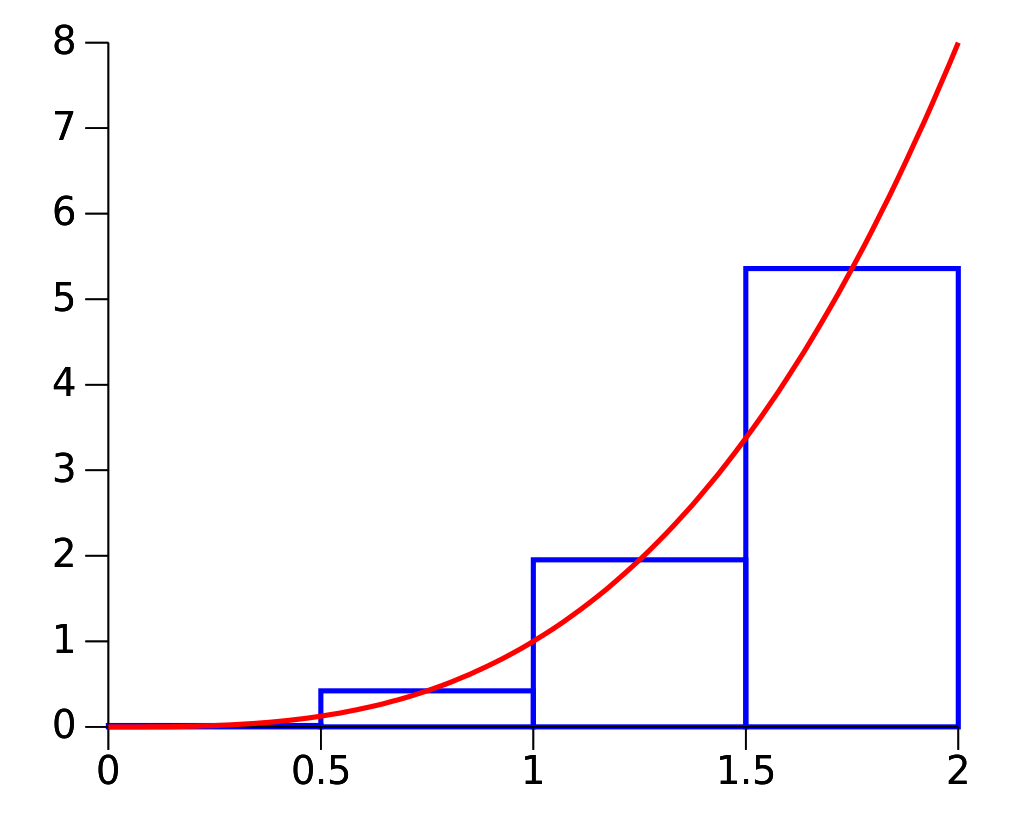
\includegraphics[height=3cm]{figures/MidRiemann2.svg.png}
            \caption{
                Mid-Riemann sum\footnote{\href{https://en.wikipedia.org/wiki/Riemann\_sum\#/media/File:MidRiemann2.svg}{By Qef - Own work, Public Domain, https://commons.wikimedia.org/w/index.php?curid=7081805}}
            }
            \end{figure}
            
    \end{itemize}

\end{frame}

\begin{frame}{Gaussian Quadrature}
    $n$-point Gaussian quadrature rule yields exact results for \emph{polynomials} 
    of degree $2n - 1$ or less with a suitable choice of nodes $x_i$ and weights $w_i$, for $1 < i < n$.

    \[
        \int_{-1}^{1} f(x) \ dx \approx \sum_{i=1}^n w_i \, f(x_i)
    \]

    Examples:
    \begin{itemize}
        \item Gauss-Legendre Quadrature ($x_i$ are the roots of the Legendre polynomial)
        \item Chebychev-Gauss Quadrature ($x_i$ are the Chebychev nodes)
        \item Gauss-Jacobi Quadrature ($x_i$ are the roots of the Jacobi polynomial)
    \end{itemize}
\end{frame}

\begin{frame}{Gauss-Jacobi quadrature}
    Jacobi polynomials are hypergeometric (a class of classical orthogonal polynomials).

    Approximate integrals of the form: 
    \[
        \int_{-1}^{1} f(x)(1-x)^\alpha (1 + x)^\beta \ dx    
    \]
    with $\alpha, \beta \geq -1$.

    The following are special cases of the Gauss-Jacobi quadrature rule:
    \begin{itemize}
        \item Gauss-Legendre quadrature with $\alpha = \beta = 0$
        \item Chebychev-gauss quadrature with $|\alpha| = |\beta| = \frac{1}{2}$
        \item Gauss-Gegenbauer quadrature with $\alpha = \beta$
    \end{itemize}
\end{frame}

\begin{frame}{Orthogonal Polynomials and their Recurrence relation}
    \begin{itemize}
        \item \emph{Recurrence relation}: Equation that states that the $n$-th term of a sequence is equal to some combination of the previous terms.
        

            Example: \pause Fibonacci numbers: $F_n =  F_{n-1} + F_{n-2}$

            \pause

        \item \emph{Orthogonal Polynomials}: Sequence of polynomials such that any two different polynomials in the sequence are orthogonal under some inner product.
        %Only looking at the classical orthogonal polynomials (they include the Jacobi polynomials)
    
        \item Recurrence relation of classical orthogonal polynomials:
            \[
                P_n(x) = (A_n x + B_n)P_{n-1}(x) + C_n P_{n-2}(x)
            \]
    \end{itemize}
    
\end{frame}

\begin{frame}{Gauss-Jacobi Implementation: Algorithm}
    Compared implementations of GSL\footnote{\href{https://www.gnu.org/software/gsl/doc/html/integration.html\#c.gsl\_integration\_fixed\_alloc.gsl\_integration\_fixed\_type}{https://www.gnu.org/software/gsl/doc/html/integration.html}}, 
    deal.II\footnote{\href{https://www.dealii.org/developer/doxygen/deal.II/polynomial\_8h\_source.html\#l01039}{https://www.dealii.org/developer/doxygen/deal.II/polynomial\_8h\_source.html}}, 
    LehrFEM++\footnote{\href{https://github.com/craffael/lehrfempp/blob/master/lib/lf/quad/gauss\_quadrature.cc}{https://github.com/craffael/lehrfempp/blob/master/lib/lf/quad/gauss\_quadrature.cc}}
    \vspace*{0.5cm}
    \pause

    All use an iterative algorithm computing the zeros of the polynomials using the recurrence relation and Newton's method:
    \vspace*{0.25cm}
    \pause

    \begin{enumerate}
        \item Loop over the number of points/roots to compute.\pause
        \item For each one, make an (educated) initial guess, then apply Newton's method to find the root.\pause
        \item With the root, compute the weight using the gamma function.
    \end{enumerate}
    \vspace*{0.5cm}
    \pause

    This algorithm follows the implementation in LehrFEM++
\end{frame}

\begin{frame}{Quadrature Implementation: Tensor Product}
    Tensor products are used to get the quadrature nodes and weights for a reference element.

    \begin{figure}
        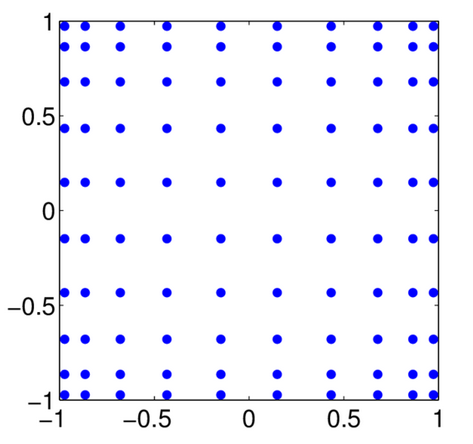
\includegraphics[height=4cm]{figures/gauss-legendre-tensor-product.png}
        \caption{Gauss-Legendre quadrature 2D tensor product\footnote{
            \href{https://www.researchgate.net/publication/284722736\_Waves\_in\_Spatially-Disordered\_Neural\_Fields\_A\_Case\_Study\_in\_Uncertainty\_Quantification}{Waves in Spatially-Disordered Neural Fields: A Case Study in Uncertainty Quantification}
        }}
    \end{figure}

\end{frame}

\section{Future}

\begin{frame}{Plan for the (near) Future}
    \begin{itemize}
        \item Finish Building Blocks: 3D

        \item FEMPoissonSolver
        
        \pause

        \item Writing
        \item Unit testing: Gauss Jacobi, 3D implementations
        \item Documentation
        
        \pause

        \item Higher-order (equidistant) Lagrange
    \end{itemize}
\end{frame}

\begin{frame}{Updated Timeline}
    \setcounter{myWeekNum}{38}
    \ganttset{%
    calendar week text={\myWeek{}}%
    }
    \begin{figure}[H]
        \centering
        \resizebox{!}{7cm}{%
        \begin{ganttchart}[
            vgrid={*{6}{draw=none}, dotted},
            x unit=.08cm,
            y unit title=.6cm,
            y unit chart=.6cm,
            today={2023-11-21},%{2023-10-24},
            progress=today,
            group incomplete/.append style={fill=gray},
            group left shift=0,
            group right shift=0,
            group height=.2,
            group peaks tip position=0,
            group peaks width=1,
            group peaks height=.2,
            time slot format=isodate,
            time slot format/start date=2023-09-18]{2023-09-18}{2024-01-14}
            \ganttset{bar height=.6}
            \gantttitlecalendar{year, month=shortname, week} \\
            \ganttgroup{Familiarization}{2023-09-18}{2023-10-15} \\
            \ganttbar[bar/.append style={fill=olive}]{Researching \& Reading}{2023-09-18}{2023-10-15}\\
            \ganttbar[bar/.append style={fill=olive}]{Familiarization with IPPL}{2023-09-25}{2023-10-15}\\

            % Implementation
            \ganttgroup{Implementation}{2023-10-02}{2023-12-10} \\
            \ganttbar[bar/.append style={fill=teal}]{Building Blocks}{2023-10-02}{2023-11-26}\\
            \ganttbar[bar/.append style={fill=teal}]{Unit Testing}{2023-10-16}{2023-12-03}\\
            \ganttbar[bar/.append style={fill=teal}]{FEMPoissonSolver}{2023-11-27}{2023-12-10}\\
            \ganttmilestone[inline=false, milestone/.append style={fill=teal}]{Code Hand-in}{2023-12-22} \\

            
            % Writing
            \ganttgroup{Writing \& Presentations}{2023-10-19}{2023-12-22} \\
            \ganttmilestone[inline=false, milestone/.append style={fill=violet}]{Three Week Presentation}{2023-10-24} \\
            \ganttmilestone[inline=false, milestone/.append style={fill=violet}]{Mid-term Presentation}{2023-11-21} \\
            \ganttmilestone[inline=false, milestone/.append style={fill=violet}]{Final Presentation}{2024-01-09} \\
            \ganttbar[bar/.append style={fill=violet}]{Thesis}{2023-11-22}{2023-12-22}
        \end{ganttchart}
        }
    \end{figure}
\end{frame}

\section*{Appendix}

\begin{frame}{Appendix A: Global $\leftrightarrow$ Local Affine Transformations}

    \begin{itemize}
        \item Local to Global: $\boldsymbol{x} = \mathbf{\Phi}_K(\hat{\boldsymbol{x}}) = \mathbf{F}_K \hat{\boldsymbol{x}} + \boldsymbol{\tau}_K$
        \item Global to Local: $\hat{\boldsymbol{x}} = \mathbf{\Phi}_K^{-1}(\boldsymbol{x}) = \mathbf{F}_K^{-1} (\boldsymbol{x} - \boldsymbol{\tau}_K)$
    \end{itemize}
    
\end{frame}

\end{document}